\section{先行研究の結果}

先行研究である,Iwamuro {\it et al.}\cite{ref:9}の画像データを元に,現在使用している解析用プログラムを用いて,落下球の速度に関して解析を行った.本付録では,Iwamuro {\it et al.}\cite{ref:9}の結果に関して示す.

\subsection{落下球 解析結果}

1wt.\%PAA溶液中における球の落下速度を解析した結果をFig.\ref{fig:1-2PAA-falling}に示す.縦軸は落下速度,横軸は落下開始時からの経過時間である.超音波照射による加速が観測された.

また,超音波照射なしの状態における1から6試行目の結果をFig.\ref{fig:1-2PAA-falling1-5}に示す.また,超音波照射ありの状態における1から5試行目の結果をFig.\ref{fig:1-2onPAA-falling1-5}に,6から10試行目の結果をFig.\ref{fig:1-2onPAA-falling6-10}に示す.これらの結果から分かる通り,超音波照射ありの場合は超音波照射なしの場合と比較して値のばらつきが多く見られた.ただし,自分が行った実験結果である,Fig.\ref{fig:1PAA-falling1-5}-Fig.\ref{fig:1onPAA-falling6-10}と比較した場合,その値のばらつきは非常に小さくなっていた.

\begin{figure}[ht]
    \centering
    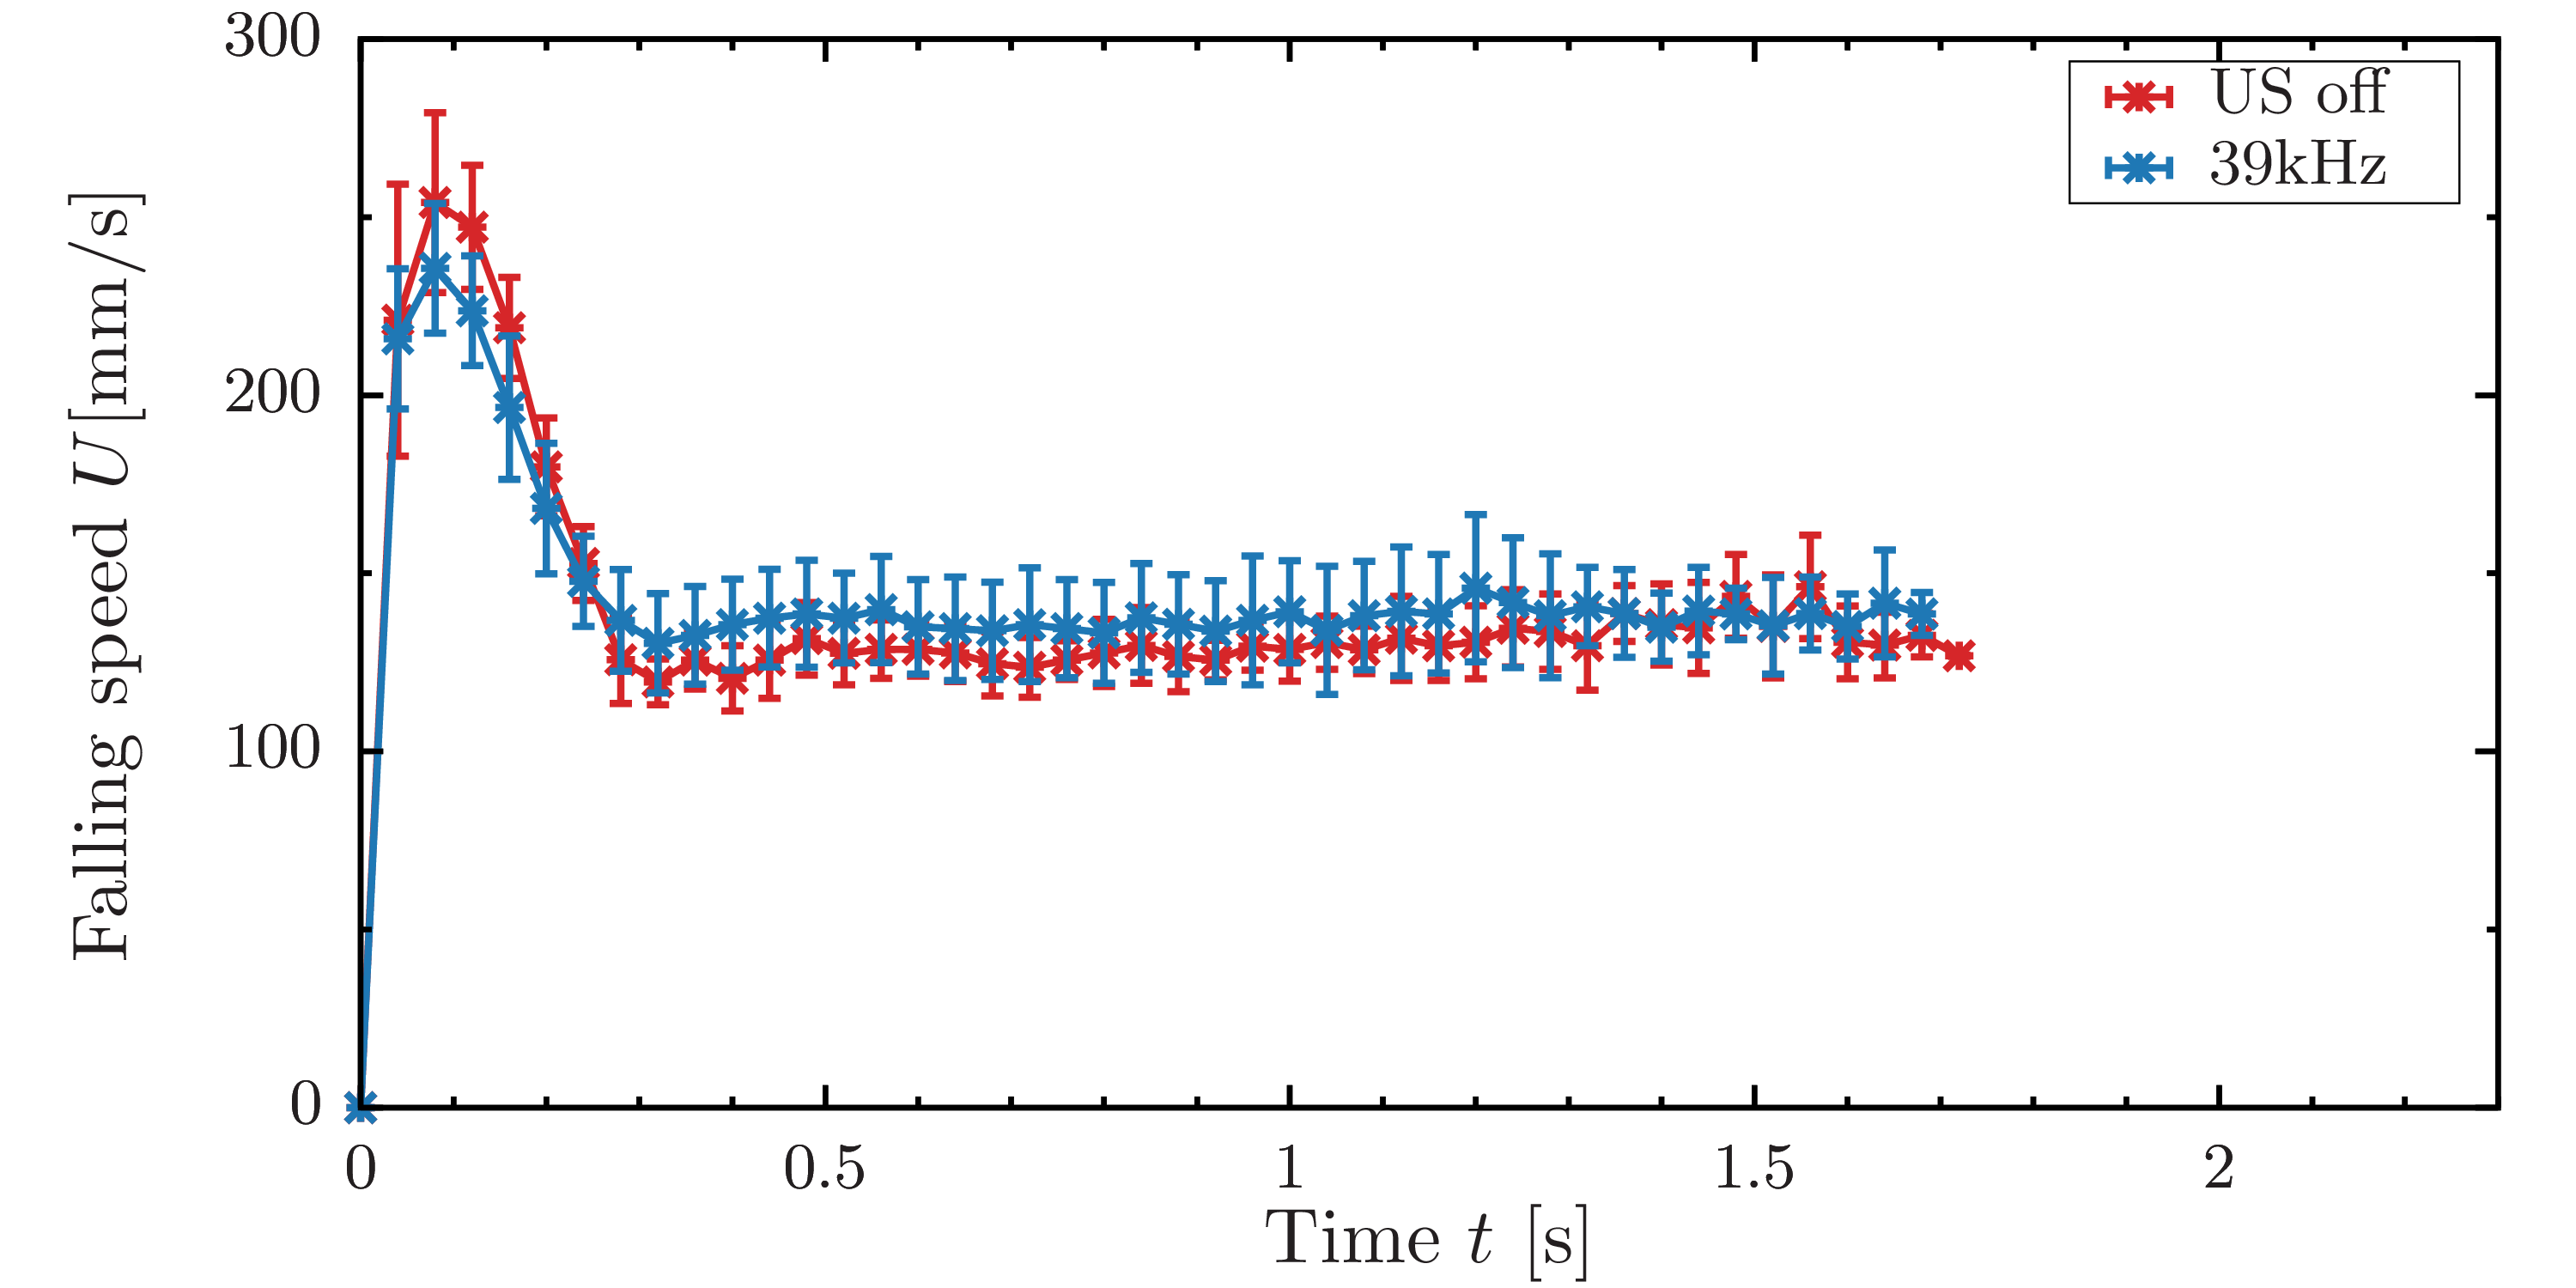
\includegraphics[width=12cm,clip]{./X-Appendix/s1-iwamuro.png}
    \caption{Falling velocity of a sphere in 1wt.\%PAA solution with and without ultrasound irradiation.}
    \label{fig:1-2PAA-falling}
\end{figure}
\begin{figure}[ht]
    \centering
    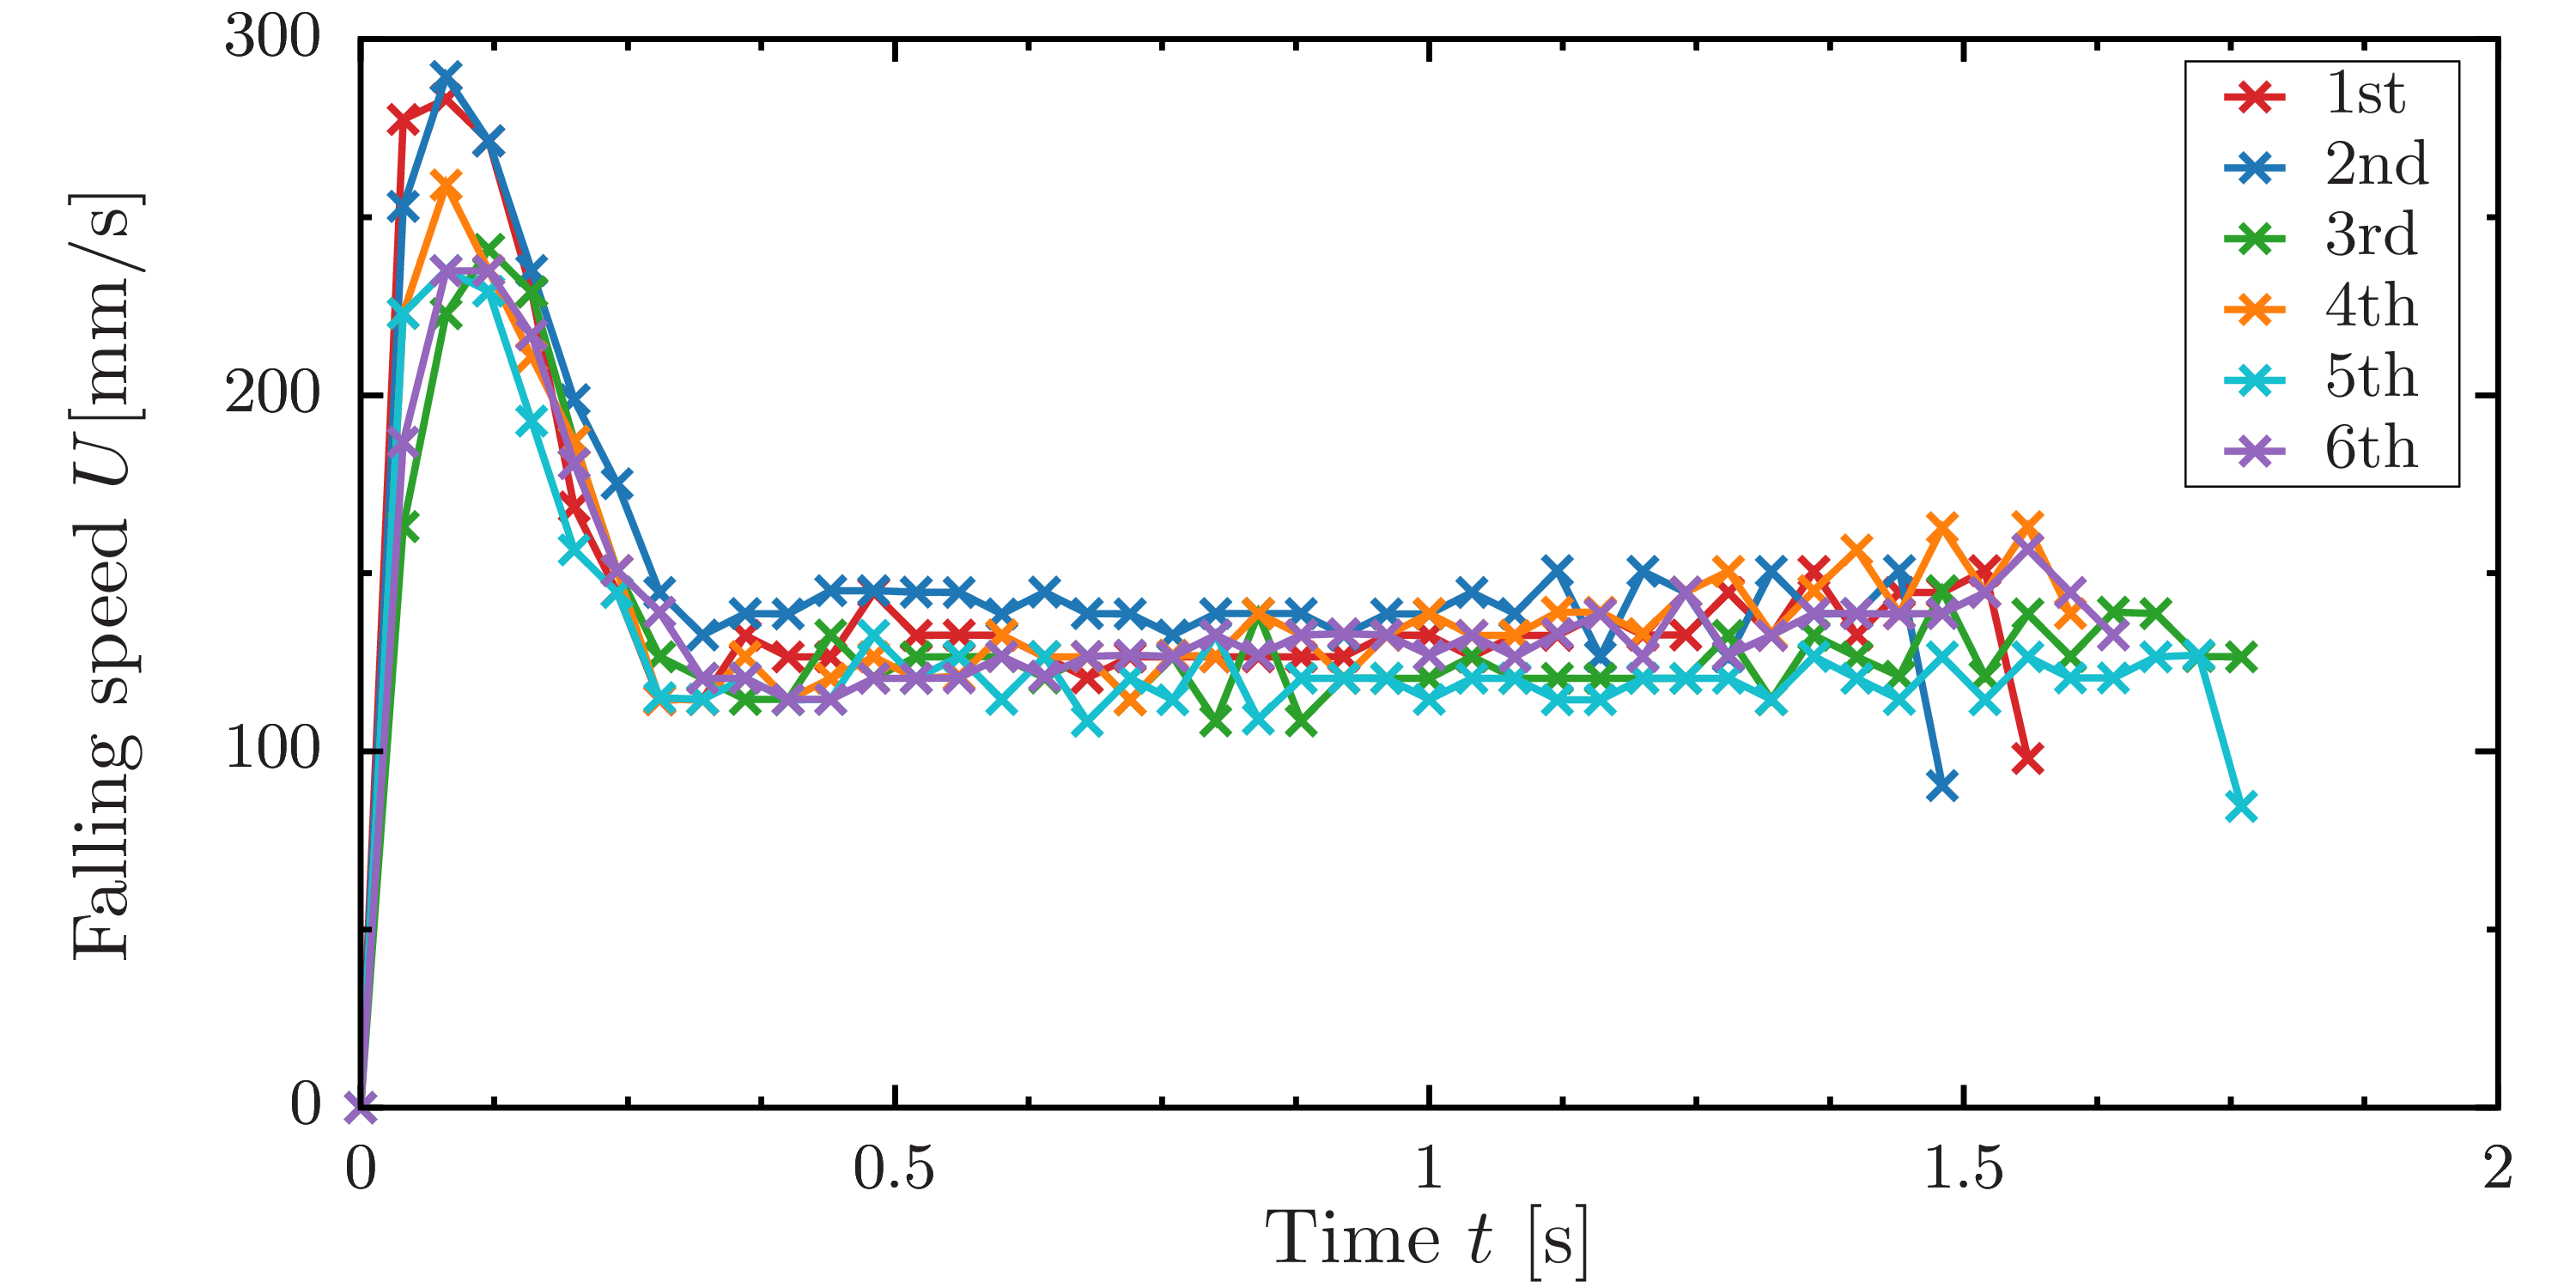
\includegraphics[width=12cm,clip]{X-Appendix/1-5.png}
    \caption{Falling velocity of the sphere for each trial (\#1 to \#6) in 1wt.\%PAA solution without ultrasonic irradiation.}
    \label{fig:1-2PAA-falling1-5}
    \centering
    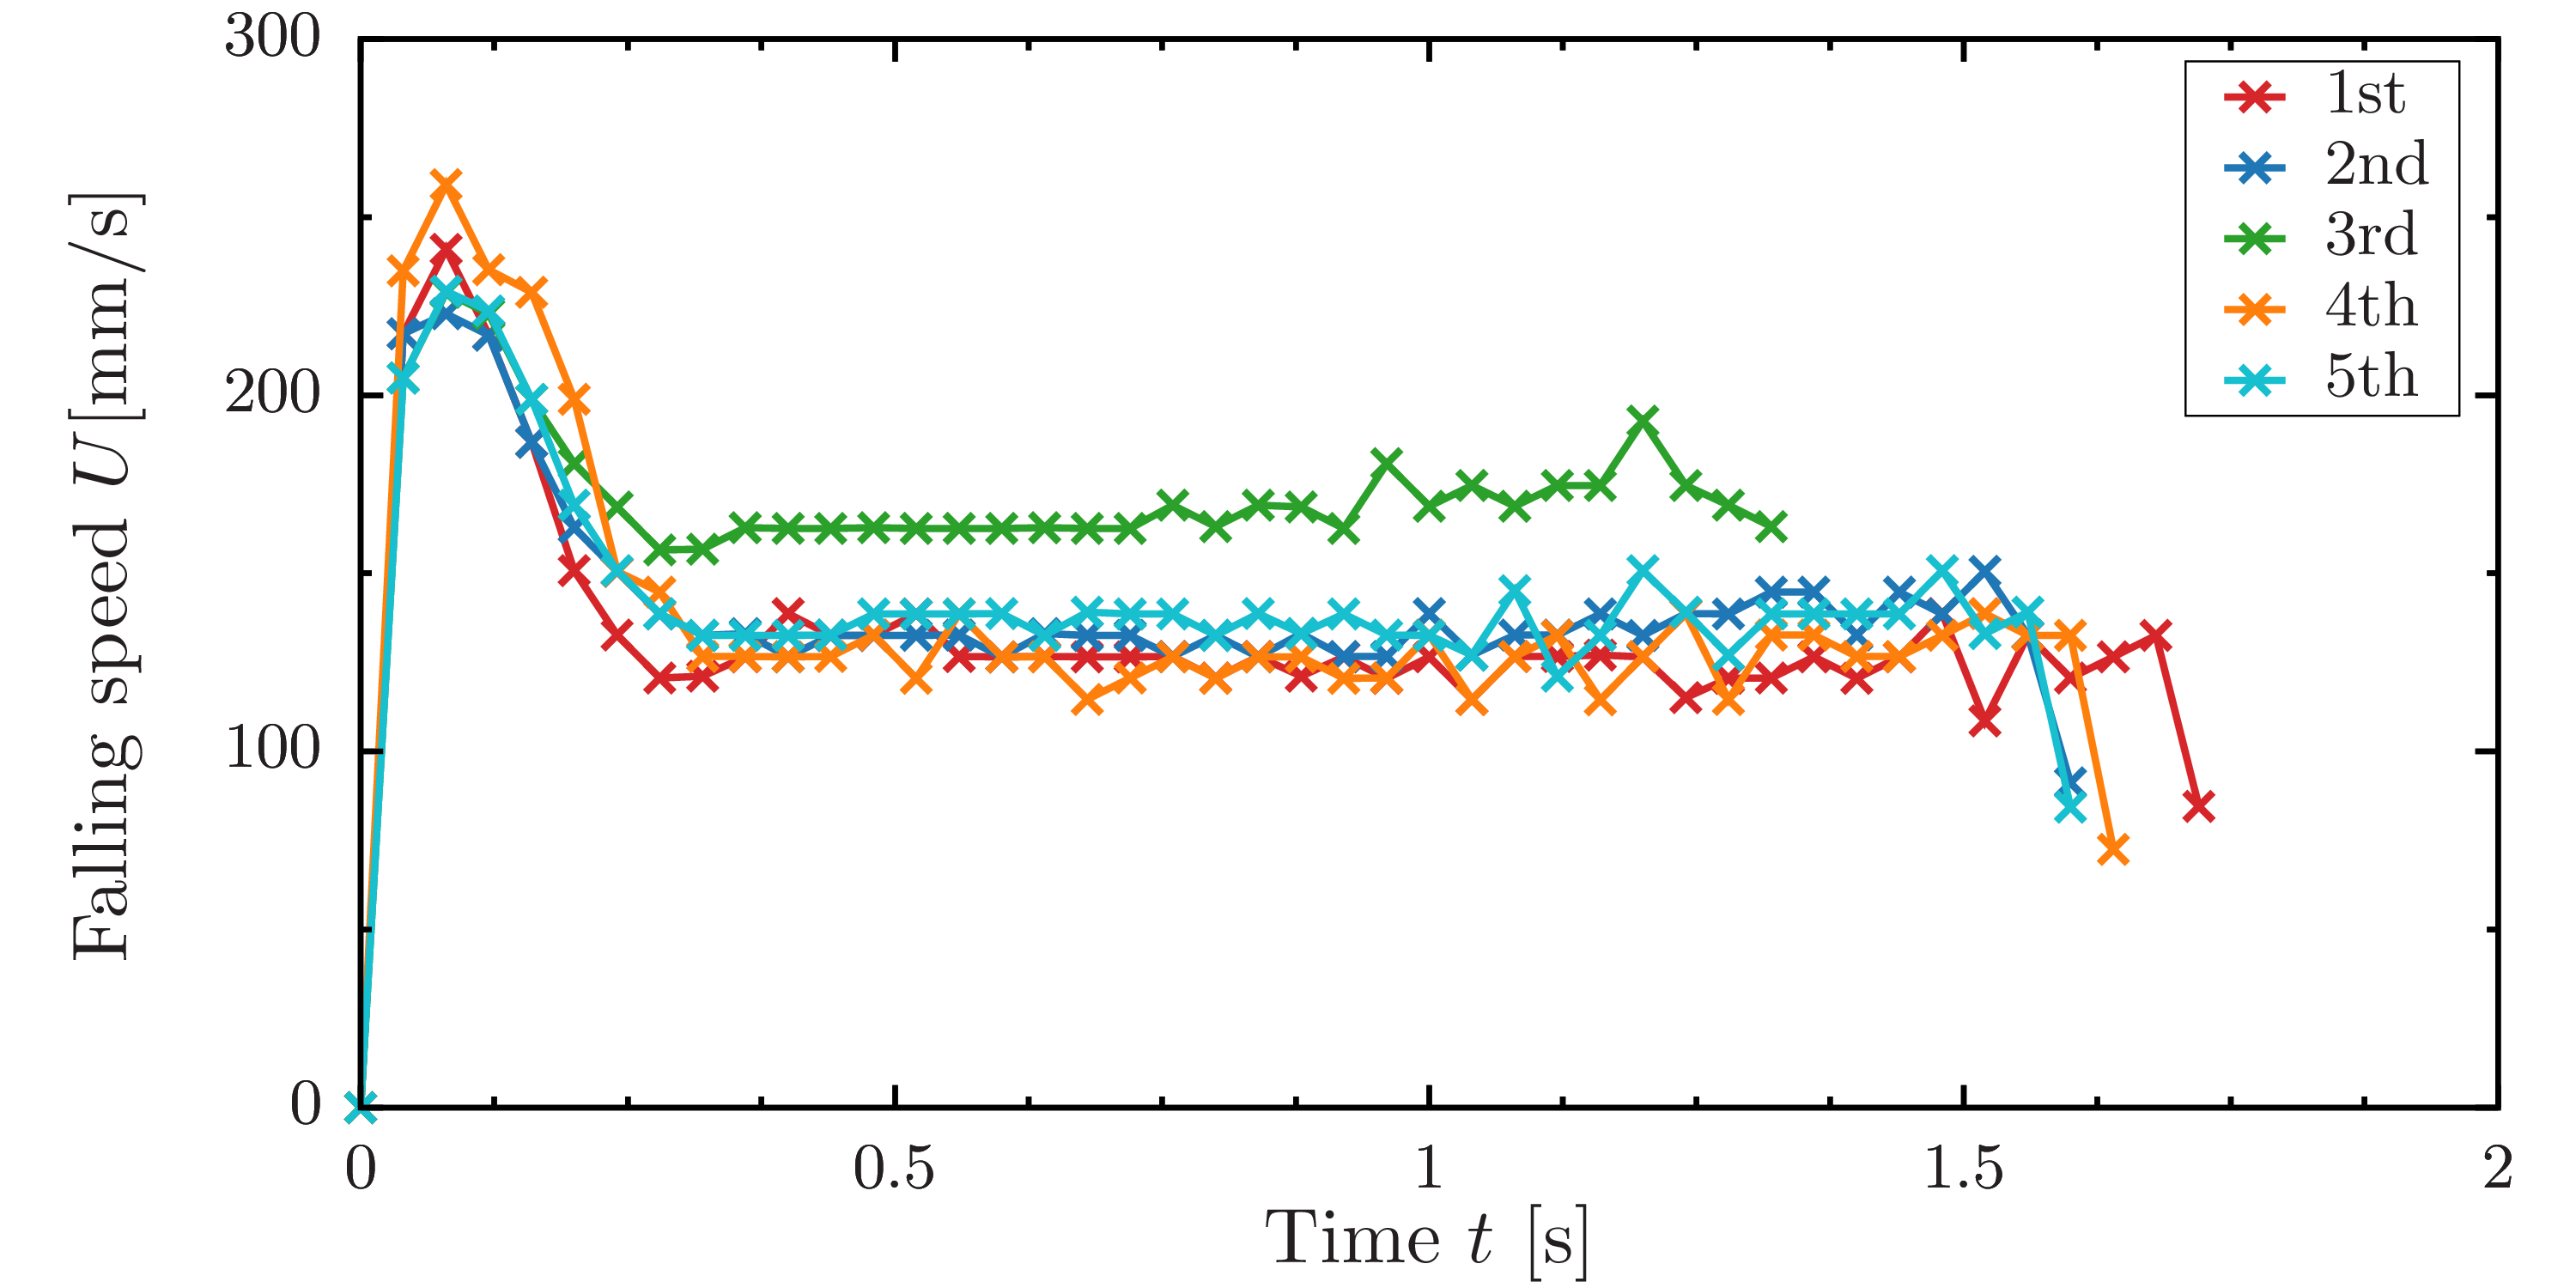
\includegraphics[width=12cm,clip]{X-Appendix/1-5-2.png}
    \caption{Falling velocity of the sphere for each trial (\#1 to \#5) in 1wt.\%PAA solution with ultrasonic irradiation.}
    \label{fig:1-2onPAA-falling1-5}
    \centering
    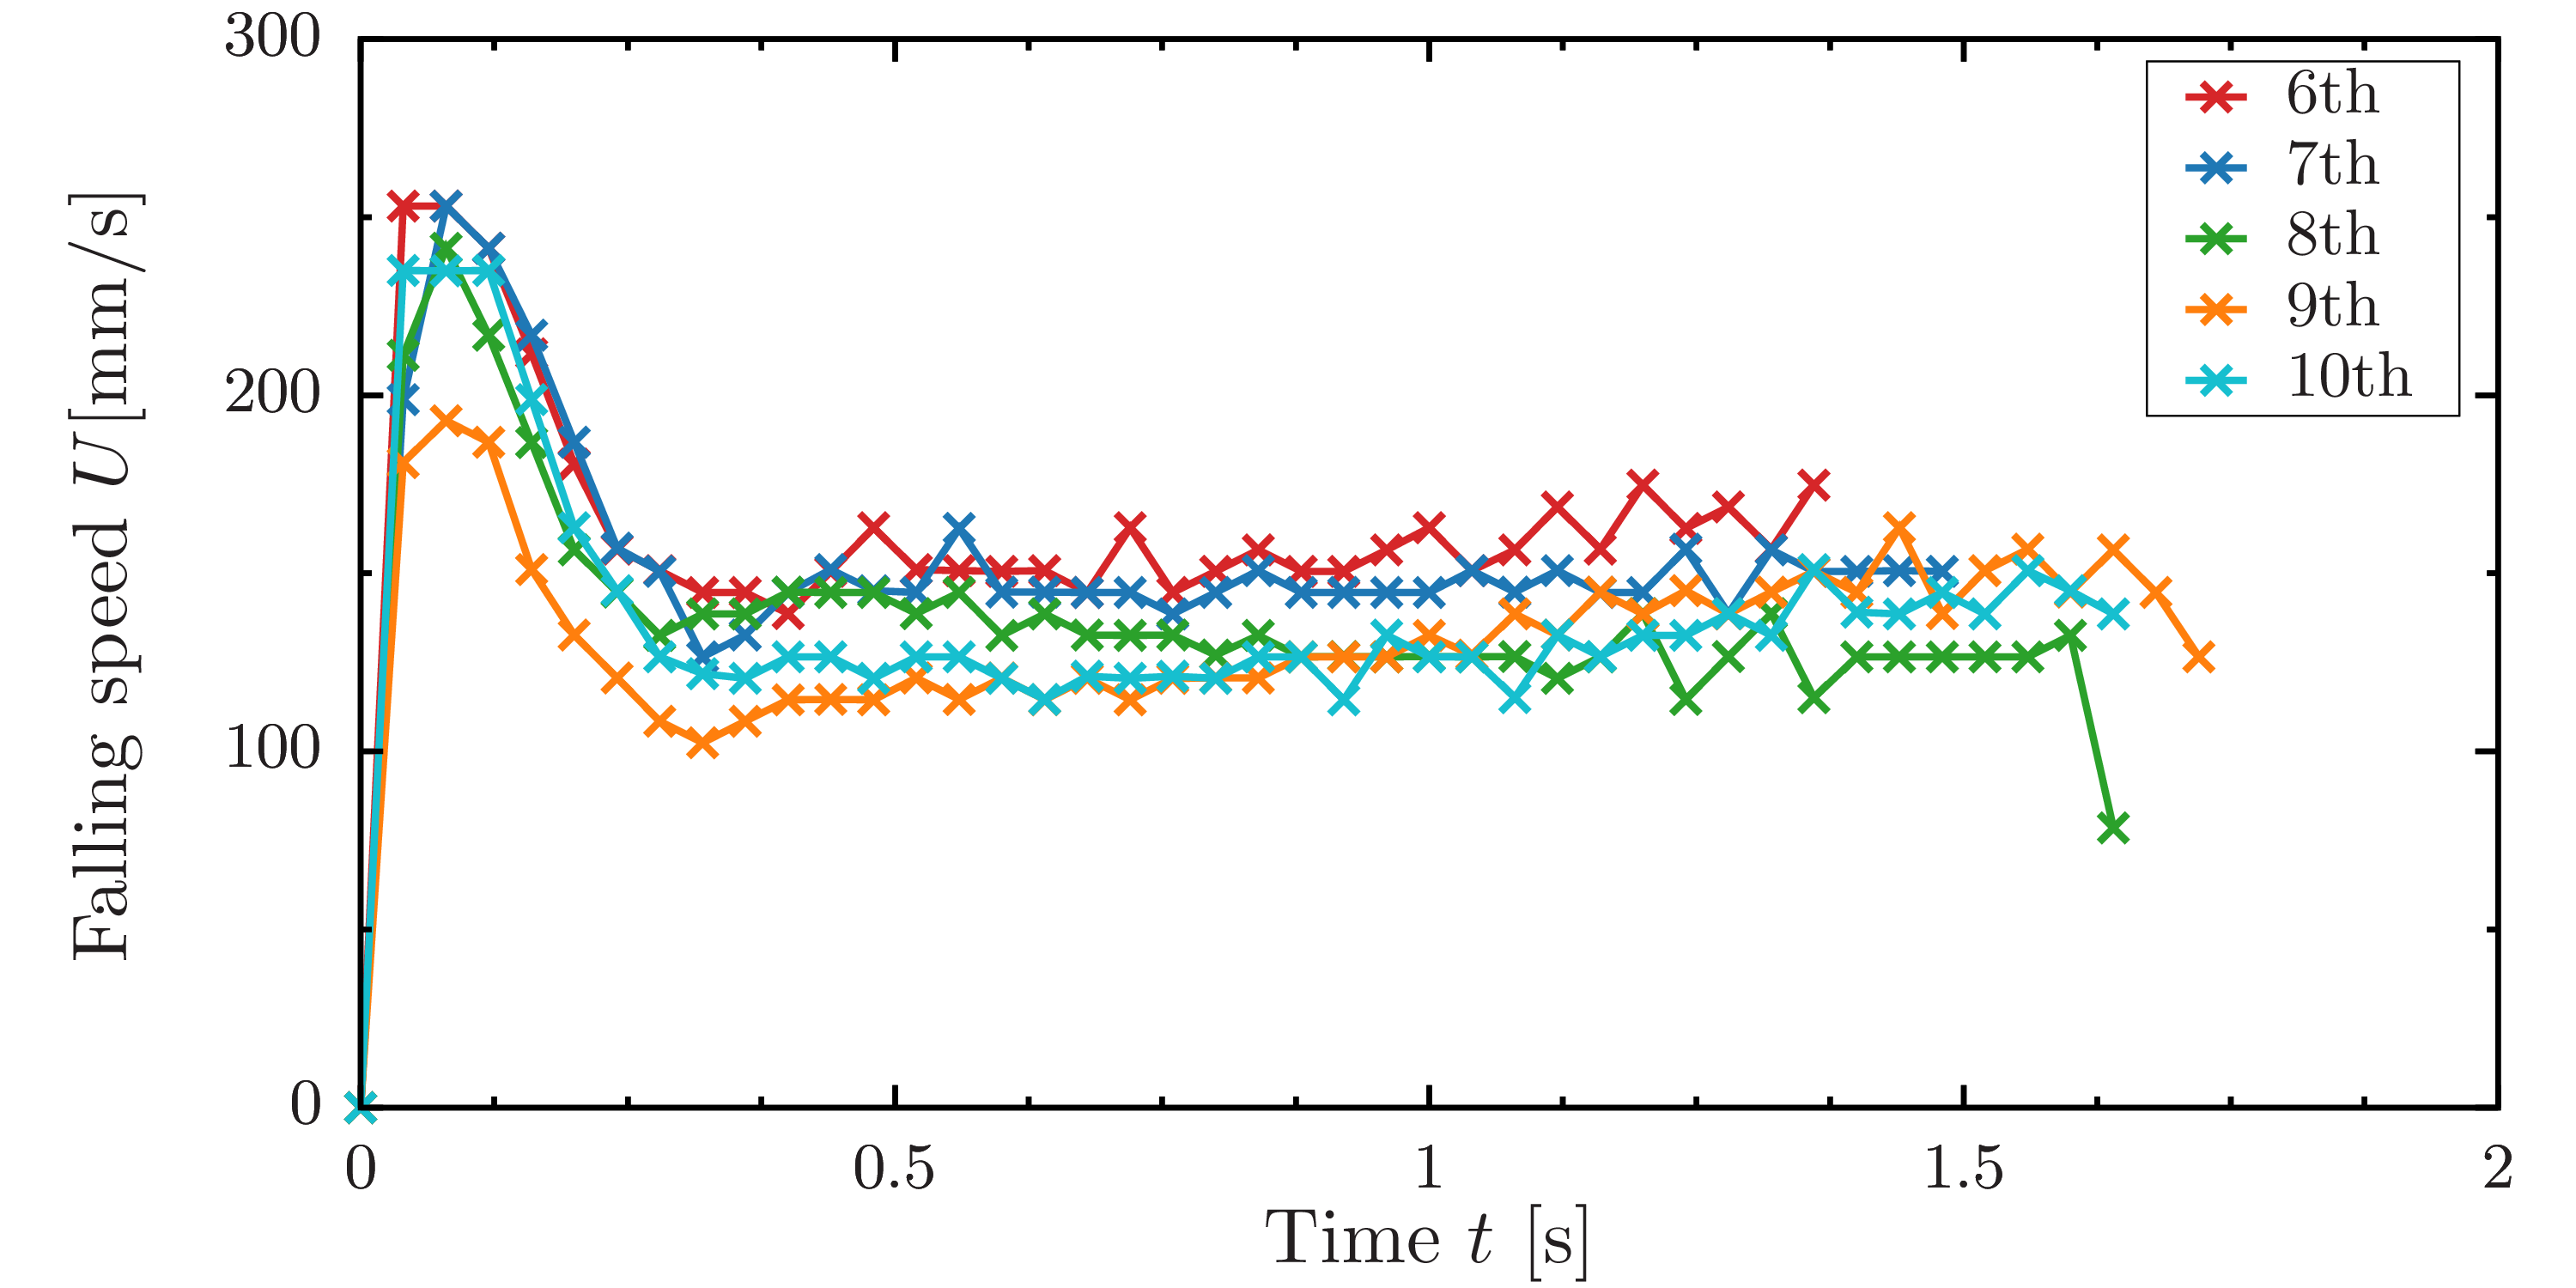
\includegraphics[width=12cm,clip]{X-Appendix/6-10.png}
    \caption{Falling velocity of the sphere for each trial (\#6 to \#10) in 1wt.\%PAA solution with ultrasonic irradiation.}
    \label{fig:1-2onPAA-falling6-10}
\end{figure}
